\documentclass[tikz]{standalone}
\usepackage[utf8]{inputenc}
\usepackage{tikz, pgfplots}
\usepackage{wasysym}
\usetikzlibrary{positioning}


\begin{document}

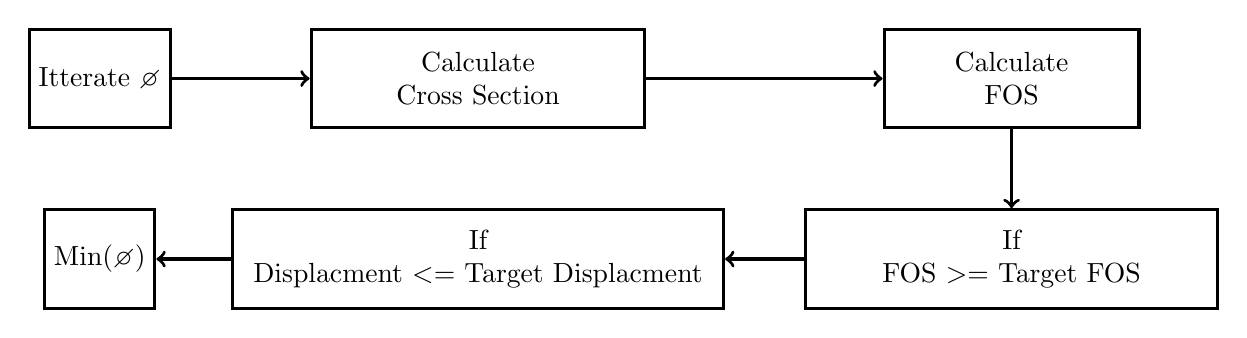
\begin{tikzpicture}[
box/.style={rectangle, draw, very thick,align=center,minimum height = 1.25cm},
]
%Nodes
\node[box](step1){Itterate \diameter};
\node[box](step2)[xshift = 0.75cm,right=of step1,text width=4cm] {Calculate \\ Cross Section};
\node[box](step3)[xshift = 2cm,right=of step2,text width=3cm]{Calculate\\ FOS};
\node[box](step4)[below=of step3,text width=5cm] {If \\ FOS $>=$ Target FOS}; 
\node[box](step5)[below=of step2,text width=6cm] {If \\ Displacment $<=$ Target Displacment}; 
\node[box](step6)[below=of step1] {Min(\diameter)}; 

%Lines
\draw[->, very thick] (step1.east) -- (step2.west);
\draw[->, very thick] (step2.east) -- (step3.west);
\draw[->, very thick] (step3.south) -- (step4.north);
\draw[->, very thick] (step4.west) -- (step5.east);
\draw[->, very thick] (step5.west) -- (step6.east);


\end{tikzpicture}

\end{document}